\chapter{Rényi Divergence and Knowledge Distillation} 

In this chapter, we begin by examining the concepts of entropy, cross-entropy, and divergence. In particular, we define Rényi divergence, establish its connection to KL divergence, and inspect some of the theoretical properties stated in \cite{vanErvenHarremoës2012}. In the second part, we formally define the notion of knowledge distillation, as proposed in \cite{HintonVinyalsDean2015}, and inspect some of the theoretical results presented therein. Furthermore, we analyze how these results change when incorporating Rényi divergence into the distillation process.

\section{KL Divergence and Rényi Divergence}

The concept of entropy, as the amount of uncertainty regarding the outcome of an experiment, was introduced by \cite{Shannon1948}.

\begin{defn}
	The entropy of a probability distribution $P = (p_1,\ldots,p_n)$ is given by
	\begin{equation*}
		H(P) = -\sum_{i=1}^{n} p_i \log p_i,
	\end{equation*}
	where we adopt the convention that $0 \log 0 = 0$.
	\label{Entropy}
\end{defn}

\begin{example}
	Let $P$ be the probability distribution of a fair coin toss, i.e., $P = (\frac{1}{2},\frac{1}{2})$. The entropy $H(P)$ is approximately $0.693$. Next, let $Q$ represent the probability distribution of an unfair coin toss, i.e., $Q = (\frac{4}{10},\frac{6}{10})$. Here, the entropy $H(Q)$ is smaller than $H(P)$, approximately $0.673$. In other words, we are less uncertain about the outcome of the unfair coin toss than about the fair coin toss.
\end{example}

To determine the similarity between two probability distributions, we cannot simply subtract their entropies. For example, the entropy of $P_1 = (\frac{4}{10},\frac{6}{10})$ is the same as the entropy of $P_2 = (\frac{6}{10},\frac{4}{10})$, yet they represent different distributions. Therefore, we use the concept of divergence, as proposed by \cite{KullbackLeibler1951}. First, we define a related notion of cross-entropy.

\begin{defn}
	The cross-entropy of a probability distribution $P = (p_1,\ldots,p_n)$ relative to another distribution $Q = (q_1,\ldots,q_n)$ is given by
	\begin{equation*}
		H(P,Q) = -\sum_{i=1}^{n} p_i \log q_i,
	\end{equation*}
	where we adopt the convention that $0 \log 0 = 0$.
	\label{Cross-Entropy}
\end{defn}

\begin{example}
	Let $P$ and $Q$ be the probability distributions as described in the example above, i.e., $P = (\frac{1}{2},\frac{1}{2})$ and $Q = (\frac{4}{10},\frac{6}{10})$. The cross-entropy of $P$ relative to $Q$ is $H(P,Q) \approx 0.714$. On the other hand $H(Q,P) \approx 0.693$  and we observe that cross-entropy is not symmetric in its arguments.
\end{example}

\begin{defn}
	The Kullback–Leibler divergence (KL divergence) of a probability distribution $P = (p_1,\ldots,p_n)$ relative to another distribution $Q = (q_1,\ldots,q_n)$ is given by
	\begin{equation*}
		D_{\text{KL}}(P \| Q) = \sum_{i=1}^{n} p_i \log \frac{p_i}{q_i},
	\end{equation*}
	where we adopt the convention that $\frac{0}{0} = 0$ and $\frac{x}{0} = \infty$ for $x>0$.
	\label{KL Divergence}
\end{defn} 

We can decompose the KL divergence into two terms, as
\begin{equation}
	\begin{aligned}
		D_{\text{KL}}(P \| Q) =& \sum_{i=1}^{n} p_i \log \frac{p_i}{q_i} \\
		=& \sum_{i=1}^{n} p_i \log p_i  + \left( - \sum_{i=1}^{n} p_i \log q_i \right), \\
		=& - H(P) + H(P, Q)
	\end{aligned}
	\label{KL_decomposition}
\end{equation}
and we observe that cross-entropy can be decomposed into entropy and KL divergence.

\begin{example}
	Let $P$ and $Q$ be probability distributions, given as $P = (\frac{1}{2},\frac{1}{2})$ and $Q = (\frac{4}{10},\frac{6}{10})$. From the previous examples, we know that $H(P) \approx 0.693$ and $H(P,Q) \approx 0.714$. Using Equation~(\ref{KL_decomposition}), we can calculate the KL divergence of $P$ relative to $Q$ as $D_{\text{KL}}(P \| Q) = - H(P) + H(P, Q) \approx 0.021$.
\end{example}

Kullback–Leibler divergence was later generalized by \cite{Rényi1961}. We begin with the definition.

\begin{defn}
	The Rényi divergence of order $\alpha$ of a probability distribution $P = (p_1,\ldots,p_n)$ relative to another distribution $Q = (q_1,\ldots,q_n)$ is given by
	\begin{equation*}
		D_\alpha(P \| Q) = \frac{1}{\alpha-1} \log \sum_{i=1}^{n} p_i^\alpha q_i^{1-\alpha},
	\end{equation*}
	where $\alpha$ is positive number distinct from 1, and we adopt the convention that $\frac{0}{0} = 0$ and $\frac{x}{0} = \infty$ for $x>0$.
	\label{Rényi Divergence}
\end{defn}

This definition of Rényi divergence assumes that probability distributions $P$ and $Q$ are discrete. For continuous spaces we can substitute the sum by Lebesgue integral (see \cite{vanErvenHarremoës2012}). Now, we present an example that motivated the introduction of the normalization term $\frac{1}{\alpha-1}$ in the definition.

\begin{example}
	Let $Q$ be a probability distribution and $A$ be a set, such that $Q(A)>0$. Define $P$ as the conditional distribution of $Q$ given $A$, i.e. $P(x) = Q(x|A) = \frac{Q(x)}{Q(A)}$, for $x \in A$. Now compute the Rényi divergence of $P$ relative to $Q$
	
	\begin{align*}
		D_\alpha(P \| Q) &= \frac{1}{\alpha-1} \log \sum_{x\in A} P(x)^\alpha Q(x)^{1-\alpha}, \\
		&= \frac{1}{\alpha-1} \log \sum_{x\in A} \left(\frac{Q(x)}{Q(A)}\right)^\alpha Q(x)^{1-\alpha}, \\
		&= \frac{1}{\alpha-1} \log \sum_{x\in A} \frac{Q(x)}{Q(A)^\alpha}, \\
		&= \frac{1}{\alpha-1} \log \left( Q(A)^{-\alpha} \sum_{x\in A} Q(x) \right), \\
		&= \frac{1}{\alpha-1} \log Q(A)^{1-\alpha}, \\
		&= - \log Q(A).
	\end{align*}
	In this particular example we observe that the factor $\frac{1}{\alpha-1}$ in the definition of Rényi divergence has the effect that $D_\alpha(P \| Q)$ does not depend on $\alpha$ in this example. This factor is moreover crucial in the following consideration.
\end{example}

Definition~\ref{Rényi Divergence} was formulated for orders $\alpha \in (0,1) \cup (1,\infty)$. We now show that the limits on the borders of the domain for $\alpha$ exist and therefore Rényi divergence can be naturally extended to the cases $\alpha=0,1,\infty$. That is, we inspect the limits

\begin{align*}
	D_0(P \| Q) &= \lim_{\alpha \goto 0+} D_\alpha(P \| Q), \\
	D_1(P \| Q) &= \lim_{\alpha \goto 1} D_\alpha(P \| Q), \\
	D_\infty(P \| Q) &= \lim_{\alpha \goto \infty} D_\alpha(P \| Q).
\end{align*}
where $P$ and $Q$ are discrete distributions on $\{1,\dots,n\}$. For $\alpha = 0$, we have

\begin{equation}
\begin{aligned}
		\lim_{\alpha \goto 0+} D_\alpha(P \| Q) &= \lim_{\alpha \goto 0+} \frac{1}{\alpha-1} \log \sum_{i=1}^{n} p_i^\alpha q_i^{1-\alpha}, \\
		&= - \log \sum_{i=1}^{n} \lim_{\alpha \goto 0+} p_i^\alpha q_i^{1-\alpha}, \\
		&= - \log \sum_{i=1}^{n} q_i \lim_{\alpha \goto 0+} p_i^\alpha \\
		&= - \log \sum_{i=1}^{n} q_i \, \mathds{1}\{p_i>0\},
		\label{Rényi_0}
\end{aligned}
\end{equation}
where $\mathds{1}$ is the indicator function. For $\alpha = 1$, the limit

\begin{equation*}
	\lim_{\alpha \goto 1} \frac{1}{\alpha-1} \log \sum_{i=1}^{n} p_i^\alpha q_i^{1-\alpha}
\end{equation*}
is of an indeterminate form $\dfrac{0}{0}$, allowing us to apply L'Hopital's Rule and we obtain

\begin{equation}
	\begin{aligned}
		\lim_{\alpha \goto 1} \frac{1}{\alpha-1} \log \sum_{i=1}^{n} p_i^\alpha q_i^{1-\alpha} &= \lim_{\alpha \goto 1} \frac{\sum_{i=1}^{n} p_i^\alpha q_i^{1-\alpha} \log p_i - p_i^\alpha q_i^{1-\alpha} \log q_i}{\sum_{i=1}^{n} p_i^\alpha q_i^{1-\alpha}}, \\
		&= \frac{\sum_{i=1}^{n} p_i \log p_i - p_i \log q_i}{\sum_{i=1}^{n} p_i}, \\
		&= \sum_{i=1}^{n} p_i \log \frac{p_i}{q_i}.
	\end{aligned}
	\label{Rényi_1}
\end{equation}
Lastly, for $\alpha=\infty$, we denote $Z(\alpha) = \sum_{i=1}^{n} p_i^\alpha q_i^{1-\alpha}$, and $M = \max_{i} \frac{p_i}{q_i}$ and let $j \in \{1,\dots,n\}$ be the first index at which this maximum is attained. We have
\begin{equation}
	M^\alpha q_j \leq Z(\alpha) \leq M^\alpha \sum_{i=1}^{n} q_i.
	\label{M_Inequalities}
\end{equation}
Taking the logarithm and dividing by $\alpha-1$ preserves the inequalities, as the logarithm is a monotonic function and $\alpha > 1$. From (\ref{M_Inequalities}), we obtain that
\begin{equation*}
	  \frac{\alpha log M + \log q_j}{\alpha-1} \leq \frac{1}{\alpha-1} \log Z(\alpha)  \leq \frac{\alpha log M + \log 1}{\alpha-1}.
\end{equation*}
Taking the limit $\alpha \goto \infty$
%\begin{equation*}
	%\log M = \lim_{\alpha \goto \infty} \frac{\alpha log M + \log q_j}{\alpha-1} \leq \lim_{\alpha \goto \infty} \frac{1}{\alpha-1} \log Z(\alpha) \leq \lim_{\alpha \goto \infty} \frac{\alpha log M + \log 1}{\alpha-1} = \log M.
%\end{equation*}

\begin{align*}
	\log M &= \lim_{\alpha \to \infty} \frac{\alpha \log M + \log q_j}{\alpha - 1}, \\
	&\leq \lim_{\alpha \to \infty} \frac{1}{\alpha - 1} \log Z(\alpha), \\
	&\leq \lim_{\alpha \to \infty} \frac{\alpha \log M + \log 1}{\alpha - 1} = \log M.
\end{align*}

Thus,
\begin{equation}
	\begin{aligned}
		\lim_{\alpha \goto \infty} \frac{1}{\alpha-1} \log \sum_{i=1}^{n} p_i^\alpha q_i^{1-\alpha} = \lim_{\alpha \goto \infty} \frac{1}{\alpha-1} \log Z(\alpha) &= \log M, \\
		&= \max_{i} \log \frac{p_i}{q_i}.
	\label{Rényi_inf}
	\end{aligned}
\end{equation}
The limits (\ref{Rényi_0}), (\ref{Rényi_1}) , (\ref{Rényi_inf}) allow us to define the Rényi divergences
\begin{equation*}
	\begin{aligned}
		D_0(P \| Q) &= - \log \sum_{i=1}^{n} q_i \, \mathds{1}\{p_i>0\}, \\
		D_1(P \| Q) &= \sum_{i=1}^{n} p_i \log \frac{p_i}{q_i}, \\
		D_\infty(P \| Q) &= \max_{i} \log{\dfrac{p_i}{q_i}}.
	\end{aligned}
\end{equation*}
Comparing to Definition~\ref{KL Divergence}, we see that
\begin{equation*}
	D_1(P \| Q) = D_{\text{KL}}(P \| Q),
\end{equation*}
and Rényi divergence indeed generalizes KL divergence.

Another important case of Rényi divergence is for $\alpha=\frac{1}{2}$. For only this value the Rényi divergence is symmetric, i.e., $D_{1/2}(P \| Q) = D_{1/2}(Q \| P)$. Even with this additional property, it still does not satisfy the definition of a metric, as the triangle inequality does not hold. However, Rényi divergence of order $\frac{1}{2}$ can be rewritten as a function of the squared Hellinger distance, which, as defined in \cite{Cheng2024}, for discrete probability distributions $P$ and $Q$ is given by

\begin{equation*}
	H^2(P\|Q) = \frac{1}{2} \sum_{i=1}^{n} (p_i^\frac{1}{2} - q_i^\frac{1}{2})^2.
\end{equation*}
We also get a relation
\begin{equation*}
	\frac{1}{2} \sum_{i=1}^{n} (p_i^\frac{1}{2} - q_i^\frac{1}{2})^2 = \frac{1}{2} \left( \sum_{i=1}^{n} p_i + \sum_{i=1}^{n} q_i - 2 \sum_{i=1}^{n} p_i^\frac{1}{2} q_i^\frac{1}{2} \right) = 1 - \sum_{i=1}^{n} p_i^\frac{1}{2} q_i^\frac{1}{2},
\end{equation*}
which we can use in the definition of Rényi divergence of order $\frac{1}{2}$ to express it in terms of the Hellinger distance

\begin{equation*}
	D_{1/2}(P \| Q) = \frac{1}{\frac{1}{2}-1} \log \sum_{i=1}^{n} p_i^\frac{1}{2} q_i^{1-\frac{1}{2}} = - 2 \log (1-H^2(P\|Q)).
\end{equation*}

We can also establish a connection between Rényi divergence of order $\alpha$ and $1-\alpha$ for $0 < \alpha < 1$.

\begin{align*}
	D_{1-\alpha}(P \| Q) &= \frac{1}{-\alpha} \log \sum_{i=1}^{n} p_i^{1-\alpha} q_i^{\alpha}, \\
	&=\frac{1-\alpha}{\alpha} \left( \frac{\alpha}{1-\alpha}  \frac{1}{-\alpha} \log \sum_{i=1}^{n} q_i^{\alpha} p_i^{1-\alpha} \right), \\
	&= \frac{1-\alpha}{\alpha} D_{\alpha}(Q \| P).
\end{align*}

\begin{example}
	Let us have a probability distributions $Q = (\frac{4}{10},\frac{6}{10})$ and $P = (p,1-p)$ for some $p \in [0,1]$. On the left side of Figure~\ref{fig:renyi_divergence_example}, we plot $D_\alpha(P\|Q)$ as a function of $p$, for different values of $\alpha$. Clearly when $p=\frac{4}{10}$, the divergence is zero for any $\alpha$ since both distributions are identical. Additionally, the divergence remains the same for any $\alpha$, when $p=0$ or $p=1$. This follows from the fact that $D_\alpha(P\|Q) = \frac{1}{\alpha-1} \log q_1^{1-\alpha} = - \log q_1$ when $p=1$ and $D_\alpha(P\|Q) = - \log q_2$ when $p=0$.
	
	On the right side of Figure~\ref{fig:renyi_divergence_example}, we plot  $D_\alpha(P\|Q)$ as a function of $q$, where we now set $P = (\frac{4}{10},\frac{6}{10})$ and $Q = (q,1-q)$. Again, the divergence is always equal to zero, when the distributions are identical, e.g. when $q=\frac{4}{10}$. However, for $q=0$ or $q=1$, we obtain the expression $\frac{x}{0}$ for $x>0$, which as defined in Definition~\ref{Rényi Divergence}, is set to $\infty$ for $\alpha \in (0,1) \cap (1,\infty)$. Thus, the divergence is also $\infty$. For $\alpha = 1$, the divergence is also infinite, as follows from Definition~\ref{KL Divergence}.	Interestingly, for $\alpha=0$, from (\ref{Rényi_0}) we derive that the divergence is 0, which it is for any $q$. 
	
	For other values of $\alpha$, the divergence varies, but a clear ordering emerges. That is, in the first example, the value of $D_\alpha(P\|Q)$ for $\alpha > \beta$ is greater than or equal to $D_\beta(P\|Q)$ for any $p \in [0,1]$, this is also true for the second example for any $q \in [0,1]$. Moreover, as shown by \cite{vanErvenHarremoës2012}, this holds in general, as Rényi divergence is non-decreasing in $\alpha$.
	
	Additionally, in the first example, we observe that for larger values of $\alpha$ the derivative is greater when $p$ is close to $\frac{4}{10}$, whereas it is smaller when $p$ is near $0$ or $1$. The opposite holds for smaller values of $\alpha$. Conversely, for the second example, the derivative is high as we get near $0$ or $1$, actually it converges to infinity for $\alpha>0$. As shown in the figure, the rate of this convergence is slower for small values of $\alpha$.
	 
	\begin{figure}[h!]
		\centering
		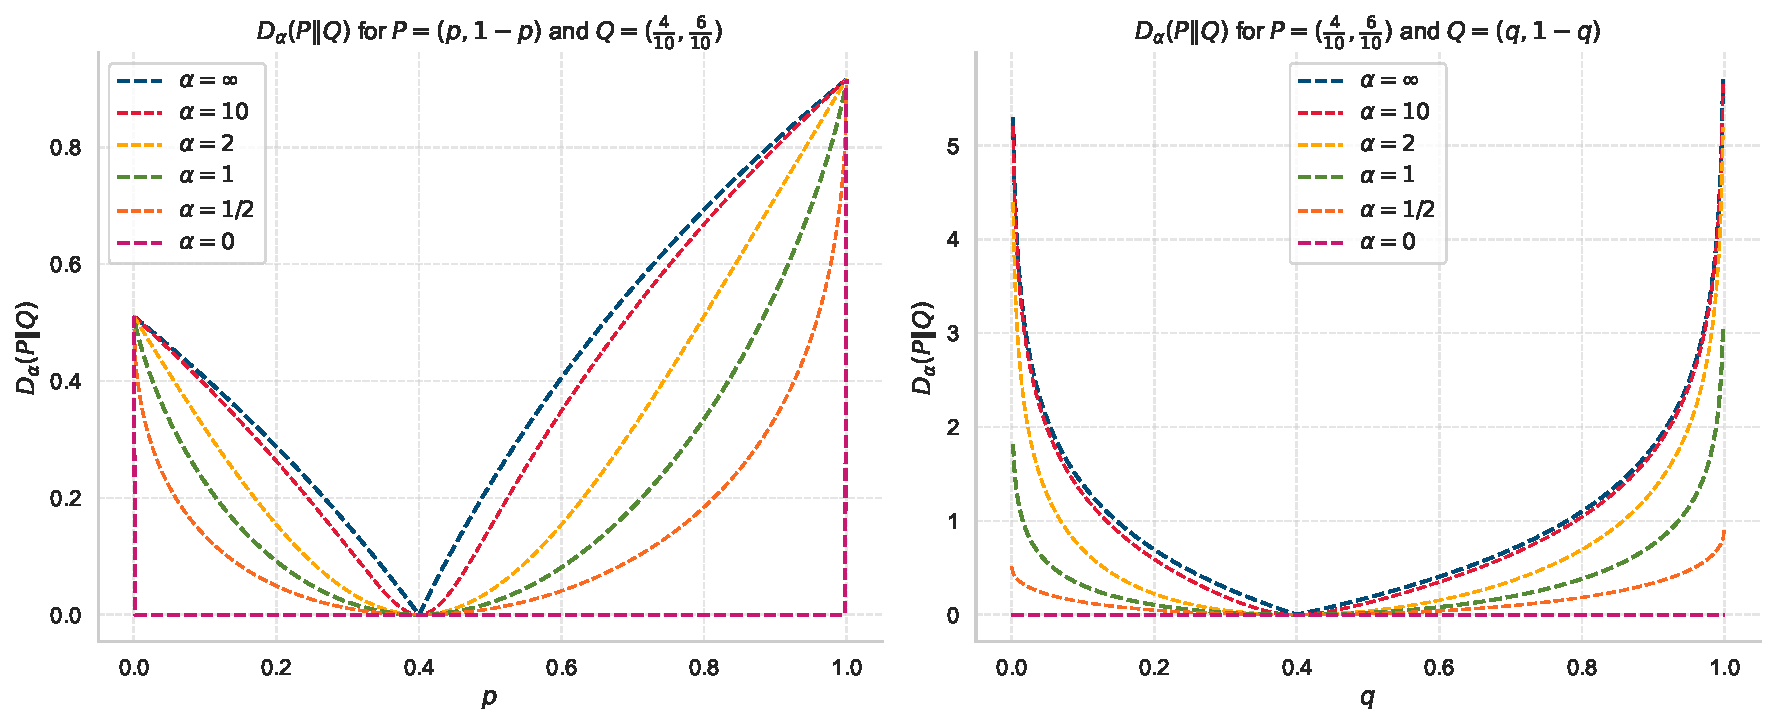
\includegraphics[width=0.9\textwidth]{../img/renyi_divergence_comparison.pdf}
		\caption{Example of Rényi divergence for a fixed distribution and another varying along the x-axis.}
		\label{fig:renyi_divergence_example}
	\end{figure}
\end{example}

The final property we focus on is the lower semi-continuity.

\begin{thm}
	Suppose we have a discrete sample space $\mathcal{Z} = \{z_1,z_2,z_3,\dots\}$ and sigma-algebra $\mathcal{A}$ is the power set of $\mathcal{Z}$. Then, for any order $\alpha \in (0,\infty]$, the Rényi divergence is a lower semi-continuous function of the pair $(P,Q)$ in the weak topology.
	\label{semicontinuity}
\end{thm}

\begin{proof}
	Let $P_1,P_2,\dots$ and $Q_1,Q_2,\dots$ be sequences of discrete distributions that weakly converge to $P$ and $Q$, respectively. We need to show
	\begin{equation*}
		\liminf_{n \goto \infty} D_\alpha(P_n \| Q_n) \geq D_\alpha(P \| Q).
	\end{equation*}
	Firstly, the weak convergence of discrete distribution $P$ means that for every bounded continuous function $h$
	\begin{equation*}
		\int h dP_n \goto \int h dP.
	\end{equation*}
	As the sample set is discrete, we may set $h=\mathds{1}\{z_i\}$ for any $i \in \N$, which is a bounded continuous function, and we obtain
	\begin{equation*}
		P_n(z_i) = \int \mathds{1}\{z_i\} dP_n \goto \int \mathds{1}\{z_i\} dP = P(z_i).
	\end{equation*}
	Now, any measurable set $A \in \mathcal{A}$ is just union of the individual elementary outcomes $z_i$  and thus the probability on any set $A$ is just the sum of the probabilities of the elementary outcomes. Using the convergence above we get
	\begin{equation*}
		P_n(A) = \sum_{z_i \in A} P_n(z_i) \goto \sum_{z_i \in A} P(z_i) = P(A),
	\end{equation*}
	and we proved that sequences $P_1,P_2,\dots$ and $Q_1,Q_2,\dots$ also converge pointwise to $P$ and $Q$, respectively. Thus, also the sequence of the pairs $(P_n,Q_n)$ converges pointwise to $(P,Q)$.
	
	Now, we can apply Fatou’s lemma term-by-term on the sum
	\begin{equation*}
		\liminf_{n \goto \infty} \sum_{i} P_n(z_i)^{\alpha} Q_n(z_i)^{1-\alpha} \geq \sum_{i} \liminf_{n \goto \infty} P_n(z_i)^{\alpha} Q_n(z_i)^{1-\alpha} \geq \sum_{i} P(z_i)^{\alpha} Q(z_i)^{1-\alpha}.
	\end{equation*}
	Taking the logarithm and scaling the by $\frac{1}{\alpha-1}$ preserves this inequality, thus yielding the lower semi-continuity of $D_\alpha(P \| Q)$.
	
\end{proof}



\section{Knowledge Distillation}

Let us define a machine learning model as a function that maps input data to output predictions

\begin{equation*}
	f_{\theta}: \mathcal{X} \goto \mathcal{Z}
\end{equation*}
where $\mathcal{X}$ is the input space, $\mathcal{Z}$ is the output space and $\theta$ is a vector representing the set of parameters of the model. In our case, as input, the model receives images from $\mathcal{X}$, where each image is represented as a tensor in $\R^{h \times w \times c}$, where $h$ and $w$ denote the height and width in pixels, respectively, and $c$ represents the number of channels, where for RGB images $c = 3$. We assume a classification task with $n$ classes, i.e., $\mathcal{Z} = \R^{n}$, so the model outputs a vector of $n$ real-valued scores, referred to as logits, given by

\begin{equation*}
	z = f_\theta(x)
\end{equation*}
for $x \in \mathcal{X}$. To convert these logits into probabilities, we use the softmax function, which is defined as

\begin{equation}
	\sigma(s)_k = \frac{e^{s_k}}{\sum_{i=1}^{n} e^{s_i}}, \qquad k = 1,2,\dots, n,
	\label{softmax}
\end{equation}
where $s \in \mathcal{Z}$. Now let

\begin{equation*}
	q_k = \sigma(z)_k, \qquad k = 1,2,\dots, n,
\end{equation*}
which represents the probability that $x$ belongs to class $k$. We denote the probability distribution produced by the model $f_\theta$ as $Q=\left(q_1,q_2,\dots,q_n\right)$. We denote by $\mathcal{Y}$ the space of such distributions, that is, $\mathcal{Y} = \{ y \in \R^n \mid y_k \geq 0 \text{ for all } k, \sum_{k=1}^{n} y_k = 1\}$. Hence, the model output $Q \in \mathcal{Y}$.

Additionally, a hyperparameter $T$, called temperature, is introduced to control the entropy of the output distribution. That is we set for $T>0$

\begin{equation}
	q_k^T = \sigma \left( \frac{z}{T} \right)_k, \qquad k = 1,2,\dots, n.
    \label{logits student}
\end{equation}
The produced probability distribution is $Q^T=\left(q^T_1,q^T_2,\dots,q^T_n\right)$. The process in called temperature scaling and popular choices for $T$ according to \cite{ChoHariharan2019} are 3, 4 and 5. Clearly, $Q^1 = Q$.

\begin{example}
	Following the example from the introduction, suppose a model $f_\theta$ that for given input yields logits for the classes \textit{horse}, \textit{zebra}, and \textit{car}, equal to 5.4, 0.2, and -1.3 respectively. In Figure~\ref{fig:temperature_example}, we see the logit values in a bar chart, along with the computed probabilities using the softmax function, both without and with temperature scaling, the latter corresponding to $T=4$.
	
	Without temperature scaling, the model is highly confident that the input belongs to the class \textit{horse} ($>0.99$), while the probabilities for the remaining classes are essentially zero. We observe that the effect of the temperature scaling is that the model is less confident about the true label while the order of the class probabilities in maintained.
	
	\begin{figure}[h!]
		\centering
		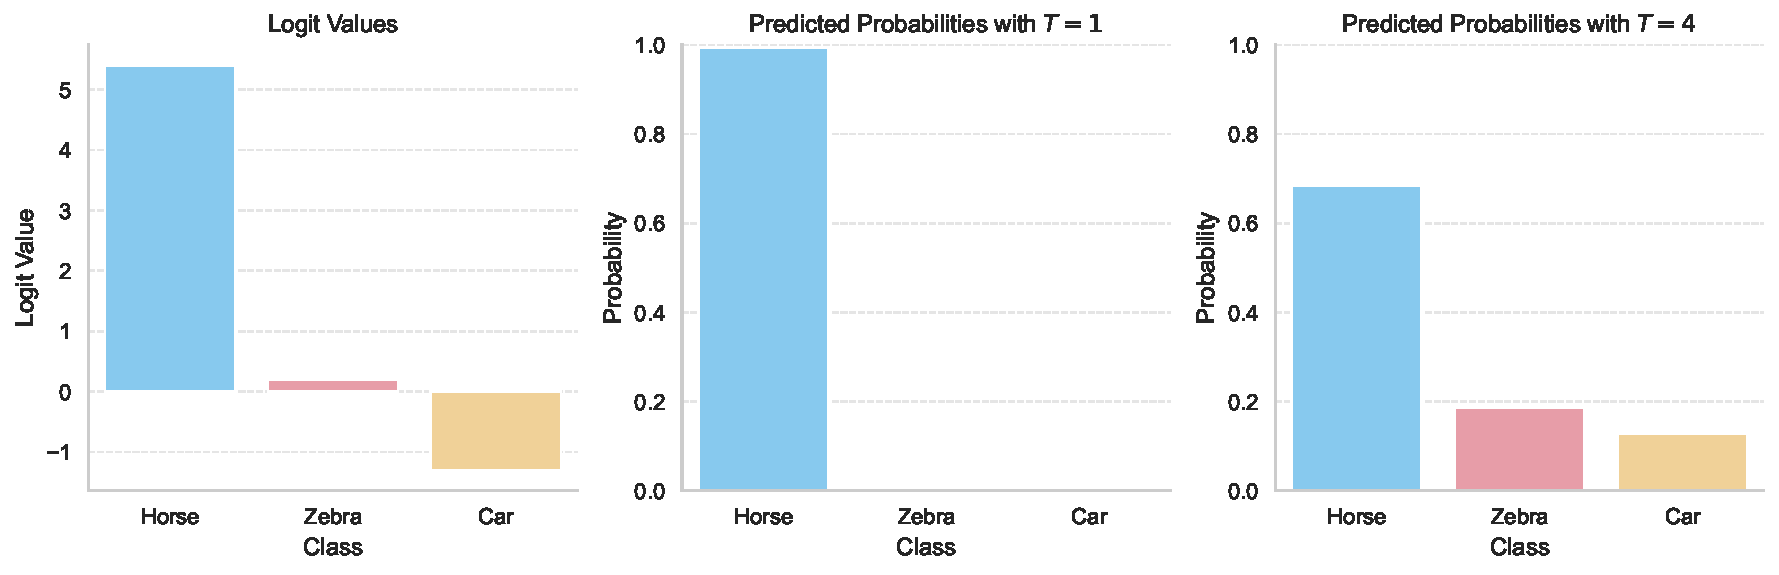
\includegraphics[width=0.9\textwidth]{../img/temperature_example_plot.pdf}
		\caption{Example of temperature scaling.}
		\label{fig:temperature_example}
	\end{figure}
\end{example}

Let $\mathcal{D}(x,y)$ denote a joint probability distribution over $\mathcal{X} \times \mathcal{Y}$, where $\mathcal{Y} = \R^n$, from which data points $(x,y)$ are independently and identically distributed (i.i.d.) samples. Now, the cross-entropy loss function $\mathcal{L_{\text{CE}}}$ is defined by

\begin{equation}
	\mathcal{L_{\text{CE}}}(\theta,x,y) = H(y \| Q) = - \sum_{j=1}^{n} y_{j} \log q_j,
	\label{Cross-entropy loss function}
\end{equation}
where $Q = (q_1,q_2,\dots,q_n)$ is the probability distribution obtained by applying the softmax function to the model's output $f(x)$, and $y_j$ is the one-hot ground-truth label, i.e., $y \in \mathcal{Y}$.

Although KL divergence provides a more intuitive measure of the difference between two distributions, being zero when the distributions are equal, unlike cross-entropy, we did not use it in Equation~(\ref{Cross-entropy loss function}). As shown in Equation~(\ref{KL_decomposition}), $H(P)$ does not depend on $Q$. Thus, the derivative of $D_{\text{KL}}(P \| Q)$ with respect to $Q$ is equal to the derivative of $H(P \| Q)$. Moreover, since cross-entropy is computationally simpler, especially when $P$ represents one-hot labels, it is often preferred over KL divergence in machine learning applications.

Training model $f_\theta$ is the process of finding the parameters $\theta$ that minimize the expected loss with respect to the distribution $\mathcal{D}$. That is, we want to find $\theta^*$ such that

\begin{equation}
	\theta^* = \arg \min_\theta \E_{(x,y) \sim \mathcal{D}} \mathcal{L_{\text{CE}}}(\theta,x,y).
	\label{vanilla_training}
\end{equation}

\begin{rem}
	In our context, the training process defined in Equation~(\ref{vanilla_training}) is referred to as vanilla training. This serves as a benchmark against which we compare our results.
\end{rem}

Knowledge distillation is a training technique where a smaller, so called student, model $f_\theta$ is trained to mimic a larger, so called teacher, model $f_t$, which has already been pre-trained. We now give a full definition.

\begin{defn}
	Suppose two models $f_\theta$ and $f_t$. Let $\mathcal{D}(x,y)$ denote a joint probability distribution over $\mathcal{X} \times \mathcal{Y}$, where $\mathcal{Y} = \R^n$, and $(x,y) \sim \mathcal{D}$. Also denote the outputs logits $z=f_\theta(x)$, which are converted into probability distribution $Q^T = (q^T_1,\dots,q^T_n)$ using softmax function introduced in Equation~(\ref{softmax}),
	\begin{equation*}
		q^T_k = \sigma \left( \frac{z}{T} \right)_k = \frac{e^\frac{z_k}{T}}{\sum_{i=1}^{n} e^\frac{z_i}{T}}, \qquad k = 1,2,\dots, n.
	\end{equation*}
	Similarly, the outputs logits $v=f_t(x)$, which are converted into probability distribution $P^T = (p^T_1,\dots,p^T_n)$ using softmax function,
	\begin{equation*}
		p^T_k = \sigma \left( \frac{v}{T} \right)_k = \frac{e^\frac{v_k}{T}}{\sum_{i=1}^{n} e^\frac{v_i}{T}}, \qquad k = 1,2,\dots, n.
	\end{equation*}
	Knowledge distillation of $f_\theta$ from $f_t$ is a training procedure in form of a minimization problem
	\begin{equation*}
		\theta^* = \arg \min_\theta \E_{(x,y) \sim \mathcal{D}} \mathcal{L}(\theta,x,y),
	\end{equation*}
	where
	\begin{equation}
		\mathcal{L}(\theta,x,y) = (1-\beta) \mathcal{L}_{\text{CE}}(\theta,x,y) + \beta \mathcal{L}_{\text{KL}}(\theta,x,y),
		\label{Knowledge Distillation Loss Function}
	\end{equation}
	where $\mathcal{L}_{\text{CE}}(\theta,x,y)$ is the standard cross-entropy loss with ground truth labels
	\begin{equation}
		\begin{aligned}
			\mathcal{L}_{\text{CE}}(\theta,x,y) &= H(y \| Q), \\
			&= - \sum_{j=1}^{n} y_{j} \log q_j,
			\label{CE loss}
		\end{aligned}
	\end{equation}
	and $\mathcal{L}_{\text{KL}}(\theta,x,y)$ is the Kullback-Leibler divergence loss with teacher's predictions
	\begin{equation}
		\begin{aligned}
			\mathcal{L}_{\text{KL}}(\theta,x,y) &= T^2 D_{\text{KL}}(P^T \| Q^T), \label{KL loss}\\
			&= T^2 \sum_{j=1}^{n} p^T_j \log \frac{p^T_j}{q^T_j},
		\end{aligned}
	\end{equation}
	$T$ and $\beta$ are hyperparameters.
	\label{Knowledge Distillation}
\end{defn}

The hyperparameter $T$ in Definition~\ref{Knowledge Distillation}  denotes temperature. During training, we apply temperature scaling to both the teacher and the student in Equation~(\ref{KL loss}). By increasing $T$, we soften the probabilities, thus retaining inter-class similarities by driving the predictions away from 0 and 1. The second hyperparameter, $\beta$, controls the balance between the cross-entropy loss and Kullback-Leibler divergence loss. A common choice for $\beta$ is $0.9$ (see \cite{ChoHariharan2019}).

%\begin{rem}
	%In many cases, the teacher model $f_t$ from Definition~\ref{Knowledge Distillation}, has been pre-trained on the same dataset $\mathcal{D}$. However, this is not always the case, for example, the teacher model may be trained on a much broader dataset or one that contains many more classes.
%\end{rem}

\begin{rem}
    The loss function in Equation~(\ref{KL loss}) includes a normalization term $T^2$, which we now elaborate on. First, we compute the derivative of the Kullback-Leibler divergence with respect to the logits of $Q^T:$
    \begin{equation}
	\begin{aligned}
		\frac{\partial D_\text{KL}(P^T \| Q^T)}{\partial z_j} &= \frac{\partial H(P^T \| Q^T)}{\partial z_j}\\
        &= - \frac{\partial}{\partial z_j}\left(\sum_{i=1}^{n} p^T_i \log \frac{e^{\frac{z_i}{T}}}{\sum_{k=1}^n e^{\frac{z_k}{T}}}\right)\\
		&= \left( \sum_{i=1}^{n} p^T_i \right)\frac{\partial}{\partial z_j}\left(\log \sum_{k=1}^n e^{\frac{z_k}{T}}\right) - \frac{\partial}{\partial z_j}\left(\sum_{i=1}^{n} p^T_i \frac{z_i}{T}\right) \\
		&= \frac{1}{T} \frac{e^{z_j}}{\sum_{k=1}^n e^{z_k}} - \frac{p^T_j}{T} \\
		&= \frac{1}{T} (q^T_j - p^T_j)
	\end{aligned}
    \label{KL gradient}
\end{equation}
If we now similarly to \cite{HintonVinyalsDean2015} assume centered logits
\begin{align}
\sum_{k=1}^{n} z_k = \sum_{k=1}^{n} v_k = 0,
    \label{centered logits}
\end{align}
we obtain by using a Taylor polynomial of order one for the exponential function
\begin{equation}
\begin{aligned}
    \frac{\partial D_\text{KL}(P^T \| Q^T)}{\partial z_j} &= \frac{1}{T} (q^T_j - p^T_j)\\
        &=\frac{1}{T} \left( \frac{e^{\frac{z_j}{T}}}{\sum_{k=1}^{n} e^{\frac{z_k}{T}}} - \frac{e^{\frac{v_j}{T}}}{\sum_{k=1}^{n} e^{\frac{v_k}{T}}} \right)\\
        &\approx \frac{1}{T} \left( \frac{1+{\frac{z_j}{T}}}{n + \sum_{k=1}^{n} {\frac{z_k}{T}}} - \frac{1+{\frac{v_j}{T}}}{n + \sum_{k=1}^{n} {\frac{v_k}{T}}} \right)\\
        &=\frac{1}{n T^2} (z_j-v_j).
\end{aligned}
	\label{additional term 1}
\end{equation}
We see that the Kullback-Leibler divergence gradient scales proportionally to $\frac{1}{T^2}$ with changing temperature $T$. Thus, we have incorporated the term $T^2$ into Equation~(\ref{KL loss}) to ensure that the relative contribution of $\mathcal{L}_{\text{CE}}(\theta,x,y)$ and $\mathcal{L}_{\text{KL}}(\theta,x,y)$ remains the same with changing temperature $T$. We also note that the approximation in Equation~(\ref{additional term 1}) is inaccurate when the temperature is small compared to the logits $z_k, v_k$. In that case, \cite{HintonVinyalsDean2015} states that the distillation pays less attention to matching logits much more negative than average. This is advantageous, as they may be significantly noisier, given that the teacher model is not penalized for them during training. On the other hand, they might convey useful information about the knowledge acquired by the teacher. Based on empirical evidence, the authors claim that ignoring large negative logits has a positive effect, as intermediate temperatures yield the best results.
\end{rem}

Now, we replace the KL divergence loss in knowledge distillation by a general Rényi divergence of order $\alpha$. 

\begin{defn}
    Assume the same setting as in Definition \ref{Knowledge Distillation}. Knowledge distillation with Rényi divergence of order $\alpha\in [0,\infty]$ is a training procedure as in Definition \ref{Knowledge Distillation} where the loss function~(\ref{Knowledge Distillation Loss Function}) is replaced by
    \begin{equation}
	\mathcal{L}(\theta,x,y) = (1-\beta) \mathcal{L}_{\text{CE}}(\theta,x,y) + \beta \mathcal{L}_{\alpha}(\theta,x,y),
	\label{Rényi Knowledge Distillation}
\end{equation}
where
\begin{equation}
	\begin{aligned}
		\mathcal{L}_{\alpha}(\theta,x,y) &= \frac{T^2}{\alpha} D_\alpha(P^T \| Q^T),\\
		&=\frac{T^2}{\alpha} \sum_{j=1}^{n} \frac{1}{\alpha-1} \log (p^T_j)^\alpha (q^T_j)^{1-\alpha}.
	\end{aligned}
	\label{Rényi loss}
\end{equation}
\end{defn}

\begin{rem}
    Similarly to above we elaborate on the normalizing factor in Equation~(\ref{Rényi loss}), which is now equal to $\frac{T^2}{\alpha}$. Our aim is to compute the derivatives of $D_{\alpha}(P^T \| Q^T)$ with respect to the logits of $Q^T$ for $\alpha\notin \lbrace 0,1,\infty\rbrace$ and to derive an analogous expression to Equation~(\ref{additional term 1})\footnote{Similar results as below hold to the remaining cases $\alpha\notin \lbrace 0,1,\infty\rbrace$ and can be shown using limiting procedures.}. First, recall the relation of the logits $z_k$ and probabilities $q_k$ in Equation~(\ref{logits student}) and denote
    \begin{equation*}
        Z_\alpha = \sum_{i=1}^{n} p_i^\alpha q_i ^{1-\alpha} = \sum_{i=1}^{n} p_i^\alpha \left( \frac{e^\frac{z_i}{T}}{\sum_{k=1}^n e^\frac{z_k}{T}} \right) ^{1-\alpha},
    \end{equation*}
    where we for simplicity omit $T$ in $P^T, Q^T, p^T$ and $q^T$. Now we calculate $\frac{\partial Z_\alpha}{\partial z_j}$:
\begin{align*}
	\frac{\partial Z_\alpha}{\partial z_j} =& \frac{\partial}{\partial z_j} \sum_{i=1}^{n} p_i^\alpha \left( \frac{e^\frac{z_i}{T}}{\sum_{k=1}^n e^\frac{z_k}{T}} \right) ^{1-\alpha}, \\
	=& \frac{\partial}{\partial z_j} p_j^\alpha \left( \frac{e^\frac{z_j}{T}}{\sum_{k=1}^n e^\frac{z_k}{T}} \right)^{1-\alpha} + \frac{\partial}{\partial z_j} \sum_{i\neq j}^{n} p_i^\alpha \left( \frac{e^\frac{z_i}{T}}{\sum_{k=1}^n e^\frac{z_k}{T}} \right) ^{1-\alpha}, \\
	=& p_j^\alpha (1-\alpha) \left( \frac{e^\frac{z_j}{T}}{\sum_{k=1}^n e^\frac{z_k}{T}} \right)^{-\alpha} \frac{\frac{1}{T} \sum_{k=1}^n e^\frac{z_k}{T} e^\frac{z_j}{T} - \frac{1}{T} e^\frac{z_j}{T} e^\frac{z_j}{T}}{(\sum_{k=1}^n e^\frac{z_k}{T})^2} \\
	& \qquad \qquad - \sum_{i\neq j}^{n} p_i^\alpha \left( \frac{e^\frac{z_i}{T}}{\sum_{k=1}^n e^\frac{z_k}{T}} \right)^{-\alpha} (1-\alpha) \frac{e^\frac{z_i}{T}}{(\sum_{k=1}^n e^\frac{z_k}{T})^2} e^\frac{z_j}{T} \frac{1}{T}, \\
	=& \frac{1-\alpha}{T} \left[ p_j^\alpha \left( \frac{e^\frac{z_j}{T}}{\sum_{k=1}^n e^\frac{z_k}{T}} \right)^{1-\alpha} \frac{\sum_{k=1}^n e^\frac{z_k}{T} - e^\frac{z_j}{T}}{\sum_{k=1}^n e^\frac{z_k}{T}} \right. \\
	& \qquad \qquad \left. - \sum_{i\neq j}^{n} p_i^\alpha \left( \frac{e^\frac{z_i}{T}}{\sum_{k=1}^n e^\frac{z_k}{T}} \right)^{1-\alpha} \frac{e^\frac{z_j}{T}}{\sum_{k=1}^n e^\frac{z_k}{T}} \right], \\
	=& \frac{1-\alpha}{T} \left[ p_j^\alpha q_j^{1-\alpha} (1-q_j) - \sum_{i\neq j}^{n} p_i^\alpha q_i^{1-\alpha} q_j \right], \\
	=& \frac{1-\alpha}{T} \left[ p_j^\alpha q_j^{1-\alpha} - q_j \sum_{i=1}^{n} p_i^\alpha q_i^{1-\alpha} \right], \\
	=& \frac{1-\alpha}{T} \left( p_j^\alpha q_j^{1-\alpha} - q_j Z_\alpha\right).
 \end{align*}
 By the chain rule and the shape of $\frac{\partial Z_\alpha}{\partial z_j}$ we have
\begin{equation}
\begin{aligned}
    \frac{\partial D_\alpha(P \| Q)}{\partial z_j}&= \frac{\partial}{\partial z_j} \left(\frac{1}{\alpha-1} \log \sum_{i=1}^{n} p_i^\alpha q_i ^{1-\alpha}\right)\\
    &=\frac{1}{\alpha-1}\frac{\partial}{\partial z_j}\left(\log Z_\alpha\right)\\
    &=\frac{1}{\alpha-1} \frac{1}{Z_\alpha} \frac{\partial Z_\alpha}{\partial z_j}\\
    &=\frac{1}{\alpha-1} \frac{1}{Z_\alpha}\frac{1-\alpha}{T}\left( p_j^\alpha q_j^{1-\alpha} - q_j Z_\alpha\right)\\
    &=\frac{1}{T} \left( q_j - \frac{p_j^\alpha q_j^{1-\alpha}}{\sum_{i=1}^{n} p_i^\alpha q_i^{1-\alpha}} \right)
\end{aligned}
\label{Rényi gradient}
\end{equation}
Using the formulas for logits of $p_j$ and $q_j$ we obtain
\begin{equation}
\begin{aligned}
    \frac{\partial D_\alpha(P \| Q)}{\partial z_j} &= \frac{1}{T} \left( q_j - \frac{p_j^\alpha q_j^{1-\alpha}}{\sum_{i=1}^{n} p_i^\alpha q_i^{1-\alpha}} \right)\\
    &=\frac{1}{T} \left[ \frac{e^{\frac{z_j}{T}}}{\sum_{k=1}^{n} e^{\frac{z_k}{T}}} -  \left( \frac{e^{\frac{v_j}{T}}}{\sum_{k=1}^{n} e^{\frac{v_k}{T}}} \right)^\alpha \left( \frac{e^{\frac{z_j}{T}}}{\sum_{k=1}^{n} e^{\frac{z_k}{T}}} \right)^{1-\alpha} \right. \\
    & \qquad \qquad \left. \left( \sum_{i=1}^{n} \left( \frac{e^{\frac{v_i}{T}}}{\sum_{k=1}^{n} e^{\frac{v_k}{T}}} \right)^\alpha \left( \frac{e^{\frac{z_i}{T}}}{\sum_{k=1}^{n} e^{\frac{z_k}{T}}} \right)^{1-\alpha} \right)^{-1} \right]
\end{aligned}
\label{complicated formula}
\end{equation}
Now we use an approximation by a Taylor polynomial of degree one. For that, we assume
\begin{align}
    \left(\frac{v_j}{T}\right)^2, \left(\frac{z_j}{T}\right)^2,\frac{v_jz_j}{T^2} \quad \text{are negligible} \quad j=1,\dots,n.
    \label{assumption negligible}
\end{align}
We also we suppose centered logits as in Equation~(\ref{centered logits}). We derive from (\ref{complicated formula}) and (\ref{assumption negligible})
\begin{align*}
	\frac{\partial D_\alpha(P \| Q)}{\partial z_j}\approx & \frac{1}{T} \left[ \frac{1+{\frac{z_j}{T}}}{n + \sum_{k=1}^{n} {\frac{z_k}{T}}} - \frac{1+{\frac{\alpha v_j}{T}}}{\left( n + \sum_{k=1}^{n} {\frac{v_k}{T}}\right)^\alpha} \frac{1+{\frac{(1-\alpha) z_j}{T}}}{\left( n + \sum_{k=1}^{n} {\frac{z_k}{T}}\right)^{1-\alpha}} \right. \\
	& \qquad \qquad \left. \left( \sum_{i=1}^{n} \frac{1+{\frac{\alpha v_i}{T}}}{\left( n + \sum_{k=1}^{n} {\frac{v_k}{T}}\right)^\alpha} \frac{1+{\frac{(1-\alpha) z_i}{T}}}{\left( n + \sum_{k=1}^{n} {\frac{z_k}{T}}\right)^{1-\alpha}} \right)^{-1} \right], \\
	=& \frac{1}{T} \left[ \frac{1+\frac{z_j}{T}}{n} - \frac{1 + \frac{\alpha v_j}{T} + \frac{(1-\alpha) z_j}{T} + \frac{\alpha (1-\alpha) v_j z_j}{T^2}}{n} \right. \\
	& \qquad \qquad \left. \left( \frac{1}{n} \sum_{i=1}^{n} 1 + \frac{\alpha v_i}{T} + \frac{(1-\alpha) z_i}{T} + \frac{\alpha (1-\alpha) v_i z_i}{T^2} \right)^{-1} \right]\\
    \approx& \frac{1}{T} \left[ \frac{1+\frac{z_j}{T}}{n} - \frac{1 + \frac{\alpha v_j}{T} + \frac{(1-\alpha) z_j}{T}}{n}\left( \frac{1}{n} \sum_{i=1}^{n} 1 + \frac{\alpha v_i}{T} + \frac{(1-\alpha) z_i}{T}\right)^{-1} \right]\\
    =&\frac{1}{T} \left[ \frac{1+\frac{z_j}{T}}{n} - \frac{1 + \frac{\alpha v_j}{T} + \frac{(1-\alpha) z_j}{T}}{n}\right]\\
    =&\frac{\alpha}{nT^2} (z_j - v_j).
\end{align*}
We have obtained
\begin{align*}
    \frac{\partial D_\alpha(P \| Q)}{\partial z_j}\approx\frac{\alpha}{nT^2} (z_j - v_j),
\end{align*}
which is a consistent formula to the case of KL divergence in (\ref{additional term 1}) which corresponds to $\alpha=1$. Also, the normalization term $\frac{\alpha}{T^2}$ in Equation~(\ref{Rényi loss}) was introduced so that the relative contribution of both terms in Equation~(\ref{Rényi Knowledge Distillation}) remains the same with changing the temperature $T$ and Rényi divergence parameter $\alpha$.
\end{rem}

\begin{rem}
If the distribution $P$ represents one-hot labels, that is $p_i=1$ for some $i\in\lbrace 1,\dots n\rbrace$, the derivative $\frac{\partial D_\alpha(P \| Q)}{\partial z_j}$ simplifies to the same form as in Equation~(\ref{KL gradient}). This holds for any choice of $\alpha$, which is why we do not modify the $\mathcal{L}_{\text{CE}}$ term in knowledge distillation or vanilla training as it would in fact have no impact on the training via stochastic gradient descent.
\end{rem}

\begin{rem}
    Lastly, let us discuss the implication of the lower semi-continuity of the Rényi divergence, as stated in Theorem~\ref{semicontinuity}, on to the goal of the Rényi divergence loss minimization in knowledge distillation. Lower semi-continuity ensures that, during the minimization process, small perturbations in the probability distribution of the student model's predictions do not lead to sudden changes in the value of the loss function. Thus, it increases the stability of the model during training, leading to smoother convergence to an optimal solution. This makes the Rényi divergence a reasonable substitution for the KL divergence.
\end{rem}

